% Standalone appendix, with its own bibliography. Build: latexmk -pdf appendix.tex
% ICLR 2027 migration of the final arXiv manuscript.
% Preliminaries and Experimental Setup are in Appendices A and B, respectively.
% Build both documents with: python3 build_papers.py
\documentclass{article}
\PassOptionsToPackage{table}{xcolor}
\usepackage{iclr2027_conference,times}
\usepackage{xr-hyper}
% Content dependencies from the arXiv manuscript, without HCL page styling.
\usepackage[T1]{fontenc}
\usepackage[utf8]{inputenc}
\usepackage{amsmath,amssymb}
\usepackage{graphicx,xcolor}
\usepackage{pifont,booktabs,adjustbox,float,multirow,wrapfig,makecell}
\usepackage[normalem]{ulem}
\usepackage{hyperref,url}
% Preserve the parenthetical role of the original numeric citation commands.
\let\cite\citep

% Keep the original figure/table palette; official ICLR layout stays unchanged.
\definecolor{hclblue}{HTML}{003366}
\definecolor{hclbrown}{HTML}{996600}
\definecolor{hclbluedark}{HTML}{00264D}
\definecolor{hclbluesoft}{HTML}{336699}
\definecolor{hclgold}{HTML}{D4A24C}
\definecolor{hclgoldsoft}{HTML}{E8C685}
\definecolor{hclink}{HTML}{1A1A1A}
\definecolor{hclinksoft}{HTML}{333333}
\definecolor{hclmuted}{HTML}{6B6B6B}
\definecolor{hclmutedtwo}{HTML}{9A9A9A}
\definecolor{hclline}{HTML}{DCE5EF}
\definecolor{hcllinestrong}{HTML}{B9C9DB}
\definecolor{hclbg}{HTML}{F8FAFC}
\definecolor{hclbgalt}{HTML}{EDF3F8}
\definecolor{hclbgsoft}{HTML}{F3F7FB}
\colorlet{hcltableheader}{hclblue!10!white}
\colorlet{hcltablegroup}{hclblue!16!white}
\colorlet{hcltablemetric}{hclblue!6!white}
\definecolor{lightpurple}{RGB}{230, 220, 235}
\definecolor{lightgreen}{RGB}{220, 230, 220}
\definecolor{lightpink}{RGB}{250, 240, 240}\providecommand{\ie}{\textit{i.e.}}
\providecommand{\eg}{\textit{e.g.}}
\DeclareRobustCommand{\inlinecolorblock}[2]{%
  \begingroup
  \setlength{\fboxsep}{0.25pt}%
  \setlength{\fboxrule}{0.35pt}%
  \raisebox{-0.15ex}{\fcolorbox{#1}{#2}{\rule{0pt}{\fontcharht\font`X}\rule{0.45ex}{0pt}}}%
  \endgroup
}


\definecolor{lotuspink}{RGB}{240,213,218}
\hypersetup{
  pdftitle={Kimodo-Policy: From Text-to-Motion Generators to Humanoid Vision-Language-Action Policies},
  pdfauthor={},
  colorlinks=true,
  linkcolor=blue,
  citecolor=blue,
  urlcolor=blue
}

\hypersetup{filecolor=blue}
\externaldocument[][nocite]{crossrefs/main_text_labels}[main_text.pdf]
\title{Kimodo-Policy: From Text-to-Motion Generators to Humanoid Vision-Language-Action Policies}
% Original author metadata retained from the arXiv final version.
% The official ICLR review mode hides this block in the rendered PDF.
\newcommand{\equalmark}{\textsuperscript{\(\star\)}}
\newcommand{\correspondmark}{\textsuperscript{\(\dagger\)}}
\newcommand{\affilmark}[1]{\textsuperscript{#1}}
\author{\parbox[t]{\textwidth}{\centering\small
Yunheng Wang\equalmark\affilmark{1}\quad
  Jiaxi Zhang\equalmark\affilmark{1}\quad
  Wei Lu\equalmark\affilmark{1}\quad
  Yuetong Fang\affilmark{1}\quad
  Taowen Wang\affilmark{1}\quad
  Yixiao Feng\affilmark{1}\\[0.3em]
  Shuning Zhang\affilmark{1}\quad
  Junzhe Xu\affilmark{1,2}\quad
  Yichi Wang\affilmark{3}\quad
  Zizhao Yuan\affilmark{1}\quad
  Kailun Huang\affilmark{1}\\[0.3em]
  Lusong Li\affilmark{2}\quad
  Mingqian Zhou\affilmark{4}\quad
  Zecui Zeng\correspondmark\affilmark{2}\quad
  Renjing Xu\correspondmark\affilmark{1}%
\\[0.6em]
\affilmark{1}\,\href{https://hkust-gz.edu.cn}{HKUST(GZ)}\quad
  \affilmark{2}\,\href{https://jd.com}{JD Explore Academy}\quad
  \affilmark{3}\,\href{https://bjut.edu.cn}{BJUT}\quad
  \affilmark{4}\,\href{https://cam.ac.uk}{University of Cambridge}
\\[0.3em]
\equalmark\,Equal contribution (co-first authors).\quad
  \correspondmark\,Co-corresponding authors.%
}}


% Keep the official anonymous review mode for this working draft.
%\iclrfinalcopy
\hypersetup{pdftitle={Kimodo-Policy: Supplementary Material}}
\begin{document}
% The official style normally sets this header inside maketitle.
\ificlrfinal
  \lhead{Published as a conference paper at ICLR 2027}
\else
  \lhead{Under review as a conference paper at ICLR 2027}
\fi
\appendix
% Generated from main_text.aux; retain numbering across both documents.
\setcounter{figure}{8}
\setcounter{table}{4}
\setcounter{equation}{2}

\section{Preliminaries}
\label{sec:preliminaries}

This section reviews the two foundations of Kimodo-Policy. We first summarize Kimodo's hierarchical text-to-motion formulation and kinematic representation (Sec.~\ref{sec:prelim_kimodo}), and then introduce ControlNet and its parameter-efficient mechanism for injecting additional conditions into a frozen diffusion backbone (Sec.~\ref{sec:prelim_controlnet}).

\subsection{Kimodo}
\label{sec:prelim_kimodo}
\textbf{Architecture Overview.} Kimodo~\cite{kimodo} is a framework for controllable kinematic motion generation based on diffusion, with pretrained models for both the SOMA~\cite{saito2026somaunifyingparametrichuman} human skeleton and the Unitree G1 humanoid robot. Starting from Gaussian noise, it generates motion sequences conditioned on text prompts and optional kinematic constraints using a two-stage Transformer denoiser operating on pose tokens. At each diffusion step $t$, its input--output mapping is summarized as
\begin{equation}
  \widehat{\mathbf{X}}_0 = \mathcal{D}_{\theta}(\mathbf{X}_t,c,t)
  = [\widehat{\mathbf{R}}_0,\widehat{\mathbf{B}}_0].
  \label{eq:kimodo_two_stage}
\end{equation}
Here, $\mathbf{X}_t$ is the noisy motion, $c$ collects the text and motion conditions, and $\widehat{\mathbf{R}}_0$ and $\widehat{\mathbf{B}}_0$ are the predicted clean root and body motions. The denoiser first predicts the global root motion, then uses its local representation to condition body prediction. Text embeddings provide semantic guidance, while masked motion constraints support control through keyframes, joint positions and orientations, and root waypoints or paths. In this work, we primarily use the Kimodo-G1 motion generation model as our pretrained backbone, which is trained on human motion-capture data retargeted to the G1 skeleton using the SOMA retargeter to enable direct generation of kinematic robot motions.

\textbf{Motion Representation.} Kimodo~\cite{kimodo} encodes a motion sequence as $\mathbf{X}=[\mathbf{x}_1,\ldots,\mathbf{x}_N]$ for $N$ frames, with the root at the first frame centered horizontally at the origin. For a skeleton with $J$ joints, each frame contains six groups of kinematic features:
\begin{equation}
  \mathbf{x}_n = [\mathbf{r}^{p}_n,\mathbf{r}^{a}_n,\mathbf{j}^{p}_n,\mathbf{j}^{v}_n,\mathbf{j}^{a}_n,\mathbf{f}_n]
  \in \mathbb{R}^{12J+9}.
  \label{eq:kimodo_motion_representation}
\end{equation}
Here, $\mathbf{r}^{p}_n\in\mathbb{R}^{3}$ is the global root position obtained by smoothing the horizontal $(x,z)$ coordinates of the pelvis while preserving its vertical height, and $\mathbf{r}^{a}_n=[\cos\psi_n,\sin\psi_n]\in\mathbb{R}^{2}$ encodes the global heading angle $\psi_n$. Joint positions $\mathbf{j}^{p}_n\in\mathbb{R}^{3J}$ use horizontal offsets from the smoothed root and absolute vertical coordinates, with axes aligned to the world frame. Joint velocities $\mathbf{j}^{v}_n\in\mathbb{R}^{3J}$ are computed from global joint positions, and joint rotations $\mathbf{j}^{a}_n\in\mathbb{R}^{6J}$ encode each joint's global orientation using a continuous 6D representation. The binary vector $\mathbf{f}_n\in\{0,1\}^{4}$ records contact states for the left heel, left toe, right heel, and right toe. These features form a root component $\mathbf{r}^{\mathrm{glob}}_n=[\mathbf{r}^{p}_n,\mathbf{r}^{a}_n]$ and a body component $\mathbf{b}_n=[\mathbf{j}^{p}_n,\mathbf{j}^{v}_n,\mathbf{j}^{a}_n,\mathbf{f}_n]$, providing an explicit decomposition for root and body motion prediction while supporting spatial constraints on root trajectories, joint positions, and joint orientations.

\subsection{ControlNet}
\label{sec:prelim_controlnet}

\textbf{Architecture Overview.} ControlNet~\cite{zhang2023adding} adapts a pretrained diffusion model to new spatial or semantic conditions while preserving the capabilities acquired by its original backbone. Its central design freezes the pretrained denoiser and adds a trainable control branch with a structurally aligned sequence of layers. The control branch processes the additional condition and produces intermediate features that are injected into the corresponding layers of the frozen branch through zero-initialized projections. For a frozen layer $F_{\ell}$, a trainable control layer $G_{\phi,\ell}$, and condition representation $\mathbf{c}$, the interaction can be written as
\begin{equation}
  \mathbf{h}^{\mathrm{ctrl}}_{\ell+1}
  =G_{\phi,\ell}(\mathbf{h}^{\mathrm{ctrl}}_{\ell},\mathbf{c}),
  \qquad
  \mathbf{h}^{\mathrm{lock}}_{\ell+1}
  =F_{\ell}(\mathbf{h}^{\mathrm{lock}}_{\ell})
  +\mathcal{Z}_{\ell}\!\left(\mathbf{h}^{\mathrm{ctrl}}_{\ell+1}\right),
  \label{eq:controlnet_prelim}
\end{equation}
where $\mathcal{Z}_{\ell}$ is a learnable $1\!\times\!1$ projection initialized to zero. At initialization, the residual path therefore contributes no signal and the adapted model exactly follows the pretrained denoiser. During optimization, gradients update only the control branch and zero projections, allowing the model to learn condition-specific behavior while retaining the original generative prior. This structure is particularly useful when the target dataset is limited or when preserving the motion regularities of a pretrained generator is important. In Kimodo-Policy, we adopt this principle for a transformer-based motion denoiser rather than a convolutional image U-Net~\cite{ronneberger2015unetconvolutionalnetworksbiomedical}. The frozen Kimodo root and body denoisers provide the motion prior, while trainable ControlNet branches receive visual features and inject residual hints at selected denoising layers. The specific visual encoder, dual-path fusion mechanism, and root/body injection strategy are described in Sec.~\ref{sec:method_architecture}.


\section{Experimental Setup}
\label{sec:experimental_setup}

This section describes the data, training protocols, and evaluation environments used to assess Kimodo-Policy. We first detail VLA policy pretraining on heterogeneous humanoid demonstrations (Sec.~\ref{sec:setup_pretraining}), and then describe post-training and evaluation on the HumanoidArena and SIMPLE simulators as well as on a physical humanoid robot (Sec.~\ref{sec:setup_posttraining}).

\subsection{Pretraining}
\label{sec:setup_pretraining}
\textbf{Dataset.} We assemble a 419-hour pretraining corpus from three publicly released humanoid datasets (Fig.~\ref{fig:pretraining_datasets}). HIW-500 provides teleoperated Unitree G1 demonstrations collected in real homes. From UniFoLM-WBT, we use the 14 task-specific G1 subsets available when our corpus was assembled: the BrainCo subsets \emph{Collect Plates into Dishwasher}, \emph{Make the Bed}, \emph{Pick Up Medicine}, and \emph{Pickup Pillow}; the Dex1 subset \emph{Put Clothes into Washing Machine}; and the Inspire subsets \emph{Clean the Living Room}, \emph{Collect Clothes (MainCamOnly)}, \emph{Pick Up Drinks}, \emph{Pickup Pillow (MainCamOnly)}, \emph{Put Clothes into Basket}, \emph{Put Clothes into Washing Machine}, \emph{Put Clothes into Washing Machine (MainCamOnly)}, \emph{Put Drinks into Fridge}, and \emph{Put Vegetables into Basket}. Main-camera-only variants are included when available, while UniFoLM-WBT entries released after this snapshot are excluded. Humanoid Everyday~\cite{humanoid_everyday} contributes 10.3K trajectories, over three million frames, and 260 tasks spanning dexterous manipulation, articulated-object interaction, human--robot interaction, and locomotion-integrated behaviors. We form training examples from an egocentric image, a language instruction, a 100-frame motion history, and a 50-frame future action chunk sampled at 30~Hz, converting trajectories to Kimodo's motion representation.

\begin{figure}[H]
  \centering
  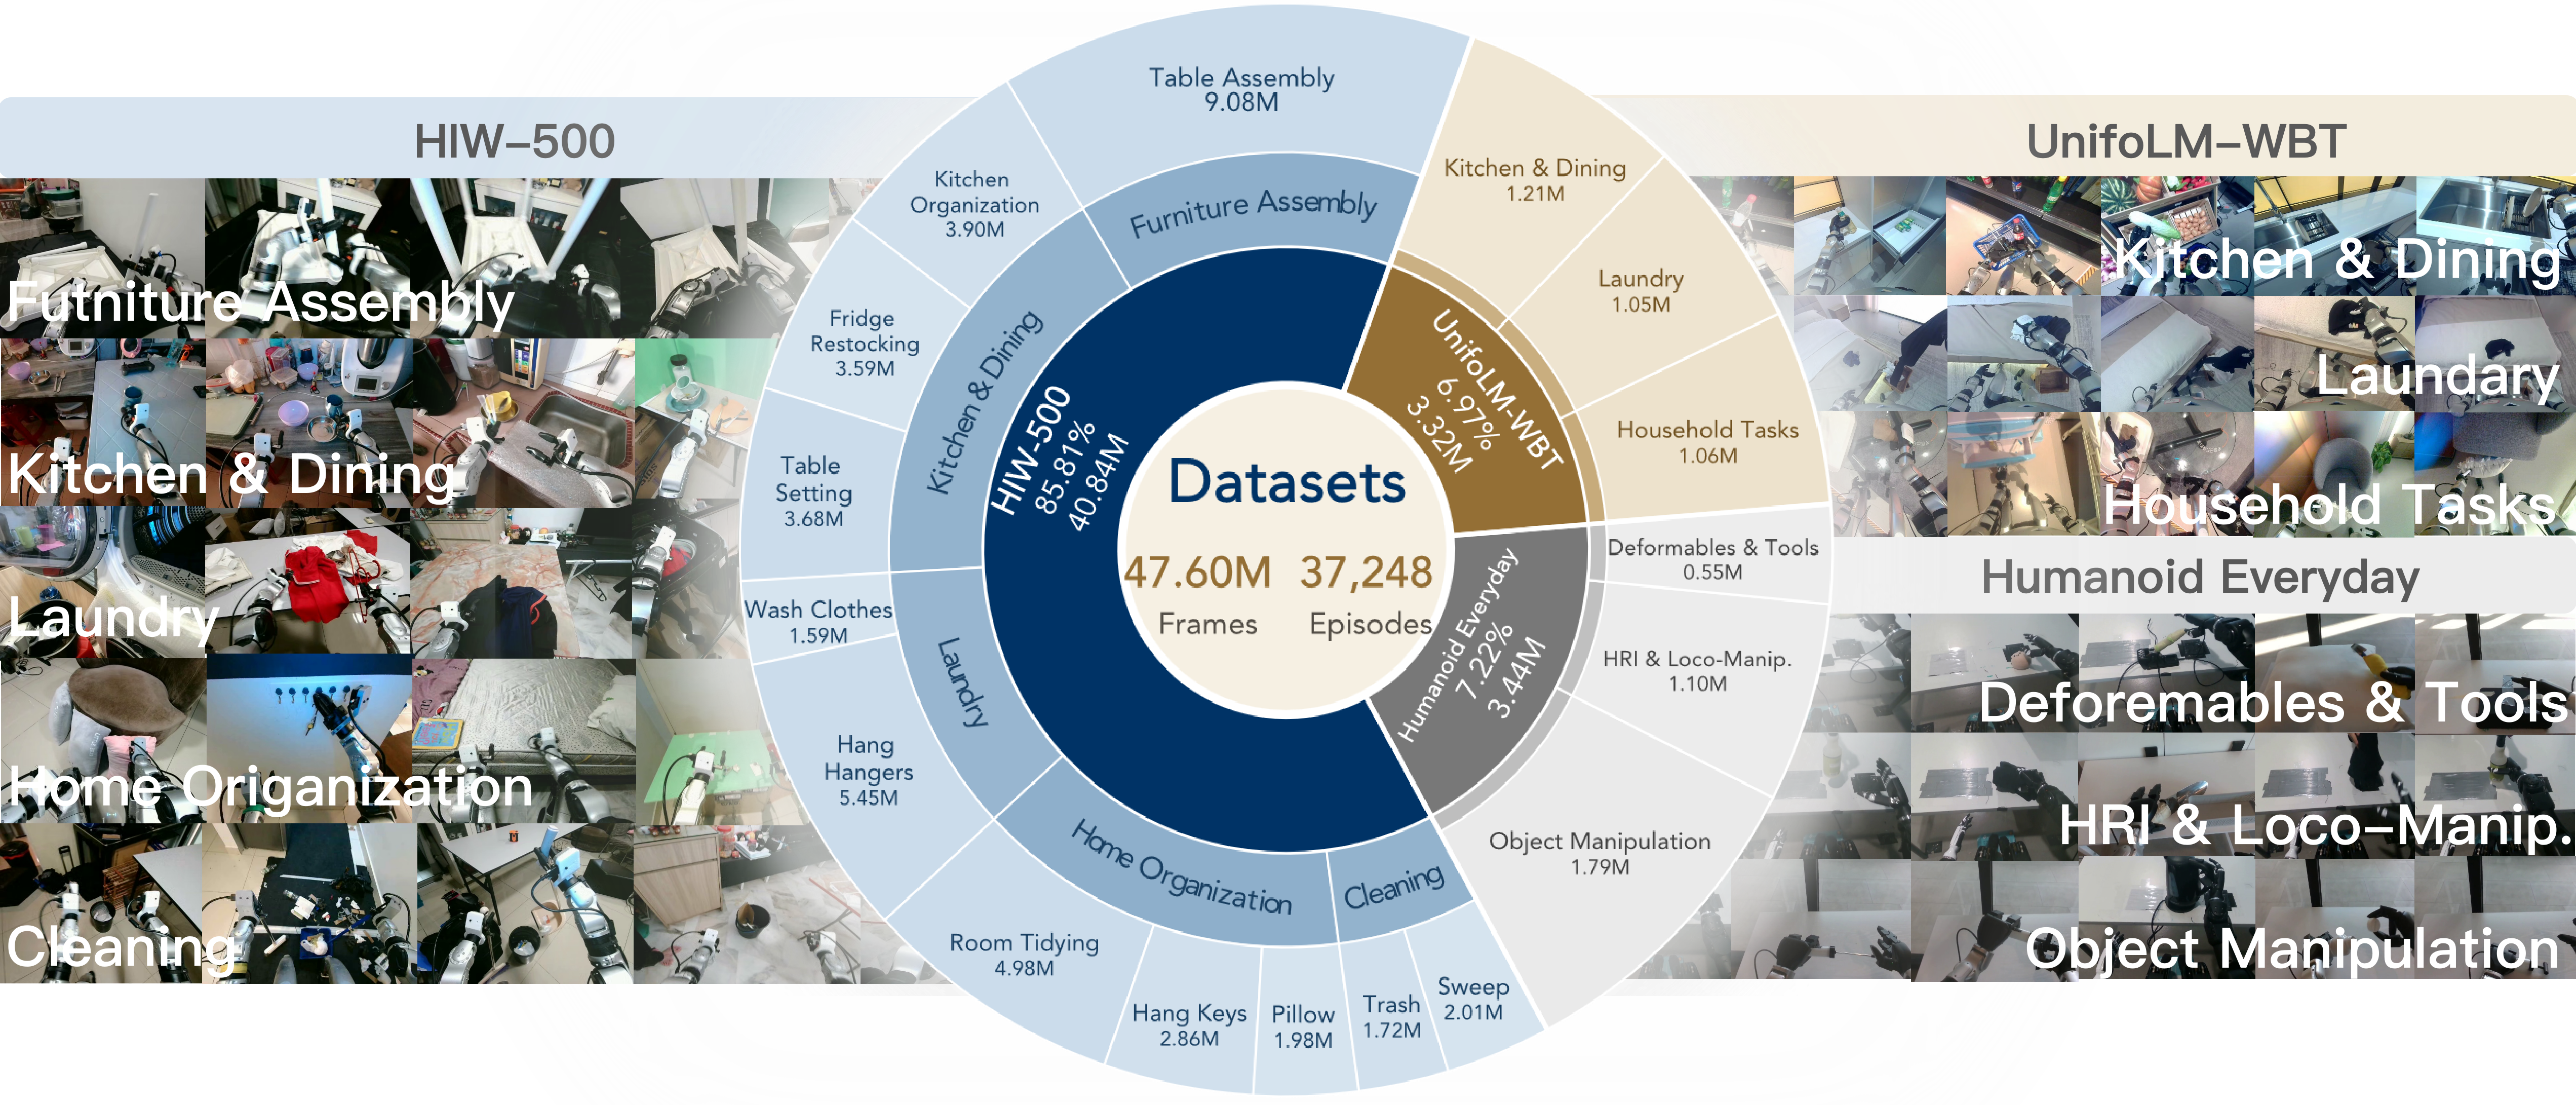
\includegraphics[width=\textwidth]{image/pretrain.png}
  \caption{\textbf{Composition of the VLA Pretraining Corpus.} The corpus combines HIW-500, 14 task subsets from UniFoLM-WBT available when the corpus was assembled, and Humanoid Everyday. UniFoLM-WBT entries released after corpus construction are excluded.}
  \label{fig:pretraining_datasets}
\end{figure}

\textbf{Implementation Details.} We pretrain the policy for 1,000k optimization steps on 16 NVIDIA H200 GPUs, taking approximately 60 hours with bfloat16 mixed precision and a global batch size of 1024. During VLA pretraining, hand supervision is represented as a two-dimensional binary vector indicating the open/closed state of the left and right hands. This shared representation accommodates the different hand morphologies, degrees of freedom, and control conventions in the source datasets, preserving grasp-and-release semantics while providing a consistent target for the hand head. We use AdamW with learning rates of $3\times10^{-5}$ for the ControlNet backbone and $1\times10^{-4}$ for the ControlNet adapters and hand head, together with a weight decay of $0.01$. The learning rate follows a cosine schedule with 1\% warm-up and a minimum of 10\% of its initial value.

\subsection{Post-Training}
\label{sec:setup_posttraining}
\textbf{HumanoidArena Benchmark.} HumanoidArena~\cite{humanoidarena,sonic} provides seven leg-critical tasks: three human--object and four human--scene interaction tasks requiring coordinated locomotion, balance, posture adjustment, and manipulation. Its SONIC data contain 100 successful demonstrations per task (700 total) with synchronized egocentric RGB, proprioceptive states, and whole-body targets. We use all seven tasks for single-task fine-tuning and joint multi-task training, the latter being more challenging because one policy must acquire all tasks simultaneously. We evaluate closed-loop performance with SONIC using success rate (SR) and average fall rate (AFR), capturing both task completion and stability during whole-body task execution.

\textbf{SIMPLE Benchmark.} SIMPLE~\cite{simple} integrates MuJoCo contact dynamics with Isaac Sim rendering for scalable evaluation of humanoid loco-manipulation. The paper describes a benchmark comprising 60 tasks; of these, 18 have been released in the public codebase to date. The paper reports baseline results for six tasks, with two evaluated using AMO and four using the SONIC tracker. From the currently released tasks, we select eight for evaluation: Handover, Mobile P\&P, XMoveBendPick, CloseDoor, OpenOven, OpenFaucet, Push Office Chair, and OpenTrashCan. Together, these tasks cover object handover, mobile pick-and-place, articulated-object interaction, and household-object manipulation, allowing us to assess policy robustness and execution stability in contact-rich whole-body control.

\textbf{Real-World Data Collection and Setup.} We collect real-world demonstrations with a teleoperation system implemented on top of and extended from the NVIDIA Isaac-GR00T data-preparation pipeline~\cite{grootn1}. As shown on the left of Fig.~\ref{fig:real_world_setup}, the operator uses a PICO 4 Ultra headset and hand controllers together with PICO body trackers for whole-body and lower-limb tracking. The humanoid is equipped with an Intel RealSense D435i camera and Dex3-1 dexterous hands. We define eight real-world tasks spanning locomotion, balance, and single- and dual-arm manipulation, and record 25--30 demonstrations per task. The two plots on the right of Fig.~\ref{fig:real_world_setup} show representative joint-position traces from two of these tasks: in Football Scoring (Fig.~\ref{fig:real_world_setup}a), the right-leg trajectory changes sharply around the kick, while in Banana Cabinet (Fig.~\ref{fig:real_world_setup}b), the traces vary across the pick, place, and push phases. In both plots, solid curves show measured joint positions and dashed curves show the corresponding action commands for the left and right sides, illustrating the task-dependent motion captured in the demonstrations. We store the demonstrations in a LeRobot v2.1~\cite{cadene2026lerobotopensourcelibraryendtoend}-compatible format, extended with Kimodo-specific motion and control fields for policy training with a motion prior.

\begin{figure}[H]
  \centering
  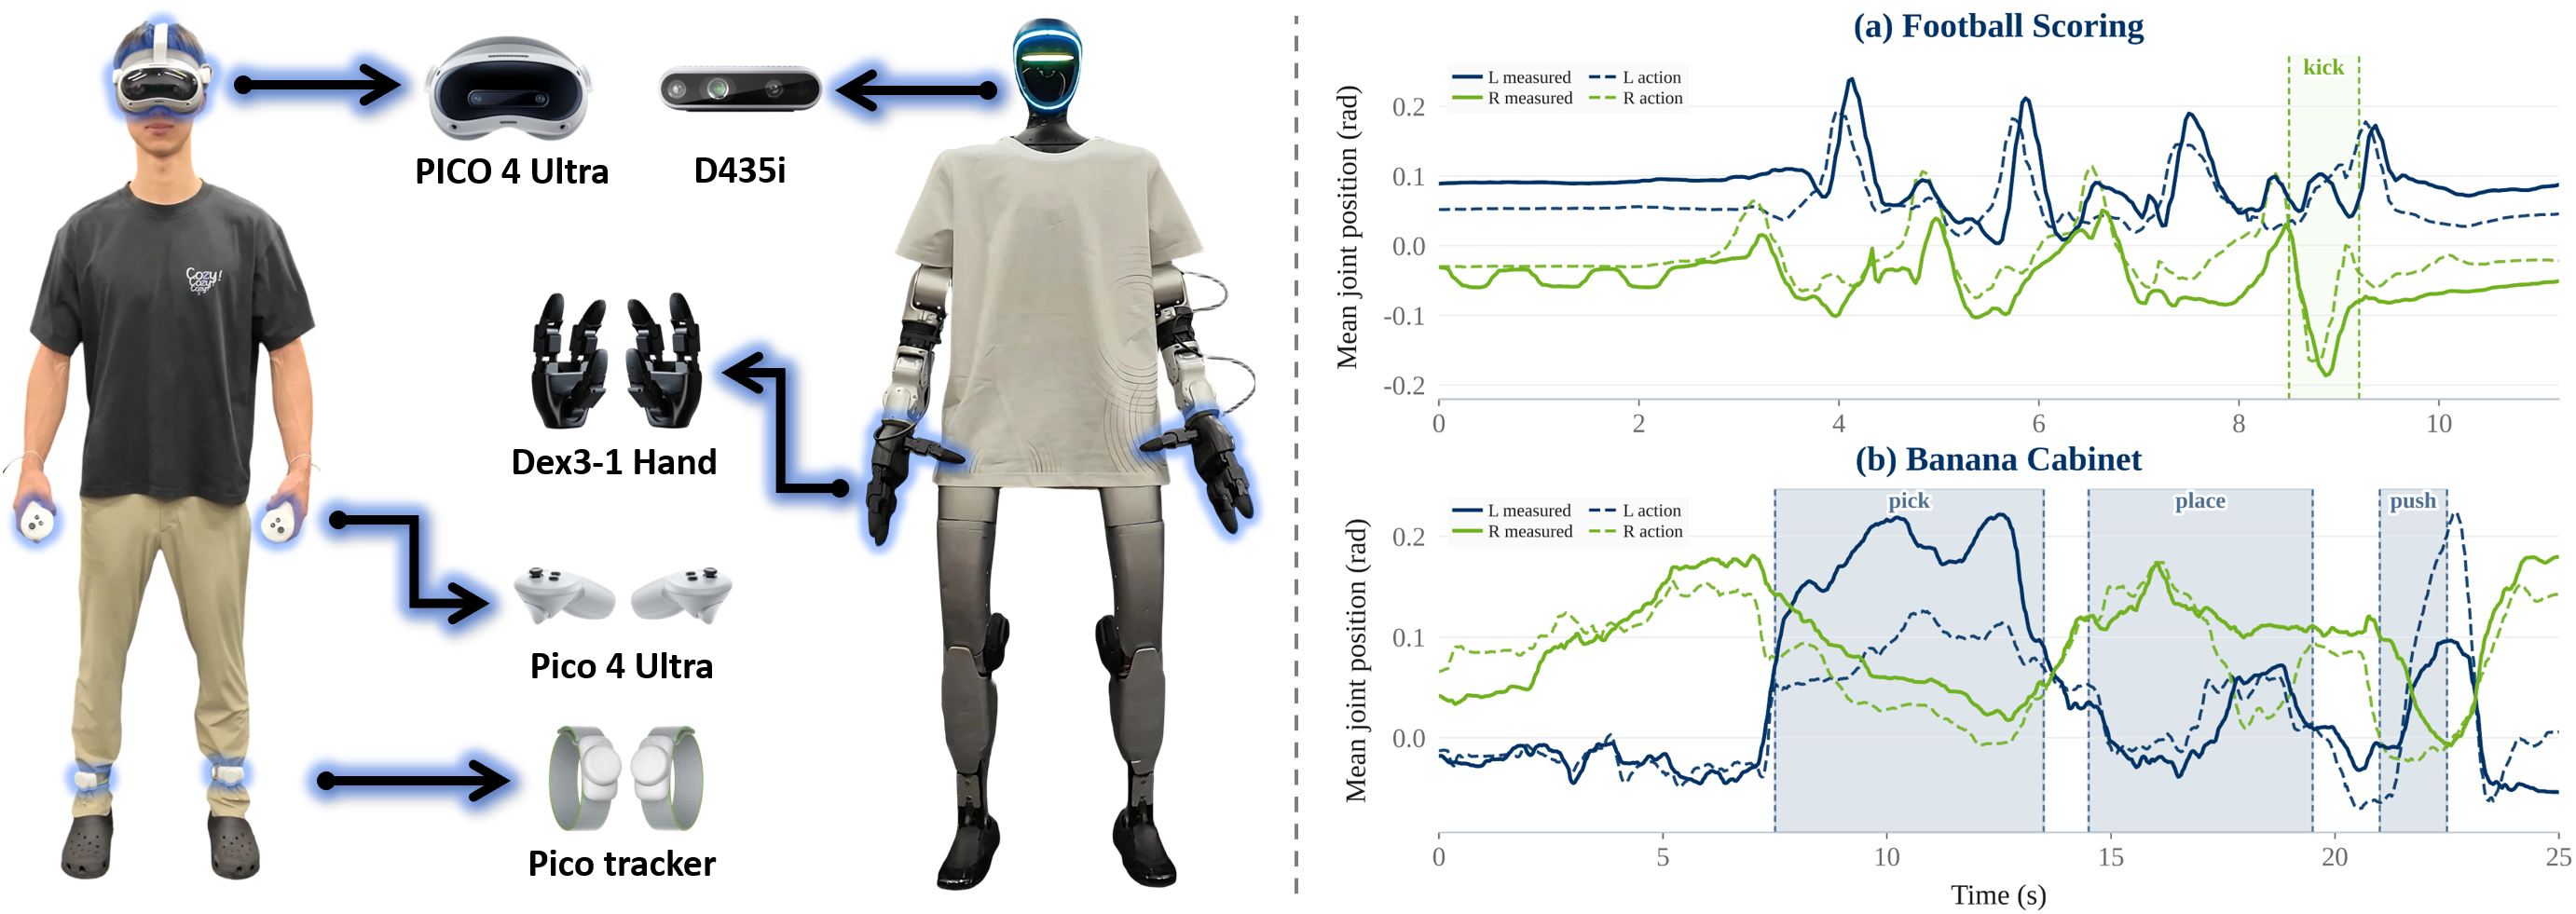
\includegraphics[width=\textwidth]{image/post-train.png}
  \caption{\textbf{Real-World Data Collection and Motion Profiles.} Left: PICO-based whole-body teleoperation of the humanoid. Right: measured (solid) and commanded (dashed) left- and right-side mean joint positions for two of the eight physical-robot tasks: (a) Football Scoring, showing a pronounced right-leg change during the kick, and (b) Banana Cabinet, showing motion across the pick, place, and push phases.}
  \label{fig:real_world_setup}
\end{figure}

\textbf{Implementation Details.} We fine-tune all policies with bfloat16 precision on four GPUs using 30\,Hz motion sequences, a 100-frame history, and a 50-frame prediction horizon. HumanoidArena single-task policies use a global batch size of 64 for 200k steps, while the joint seven-task policy uses a batch size of 128 for 500k steps; SIMPLE uses a batch size of 64 for 200k steps, and real-world policies use a batch size of 32 for 50k steps. Scratch-trained and VLA-pretrained variants share the same fine-tuning setup and differ only in initialization. The four-layer ControlNet detaches the root-control input to body prediction. We train with an MSE objective weighted 4, 1, 1, and 0.2 for root motion, body motion, hand control, and hand transitions, respectively, using AdamW (weight decay 0.01) and a cosine schedule with 1\% warm-up and a 10\% minimum learning-rate ratio. The ControlNet backbone, adapters, and hand head use learning rates of $3\times10^{-5}$, $1\times10^{-4}$, and $1\times10^{-4}$ for HumanoidArena and real-world fine-tuning, and $1\times10^{-5}$, $3\times10^{-5}$, and $3\times10^{-5}$ for SIMPLE. SIMPLE training uses color jitter and continuous hand-control targets; real-world training uses color jitter and random crops, with binary hand commands conditioned on measured hand closure. At inference, all policies run on one NVIDIA RTX 4090 with 10 diffusion denoising steps and predict a 50-frame action horizon at 30\,Hz. We execute 15 predicted frames per policy update on HumanoidArena and the real robot, and either 15 or 50 frames on SIMPLE depending on the evaluation setting. The SONIC tracker runs at 50\,Hz; real-time correction (RTC)~\cite{rtc} is enabled only for real-world deployment and disabled for HumanoidArena and SIMPLE.


\section{Task Visualizations}
\label{sec:task_visualizations}

\subsection{HumanoidArena Tasks}
\label{sec:vis_humanoidarena}

Figure~\ref{fig:humanoidarena} visualizes the seven HumanoidArena tasks through overlaid body configurations depicting successive poses. Panels (a--c) show human--object interactions involving a ball, tables, and boxes; panels (d--g) show door opening, sofa sitting, navigation, and boxing, respectively. Changes in root position and limb configuration illustrate how task execution couples locomotion, postural adjustment, and interaction with the environment. These examples contextualize the success-rate and fall-rate evaluations in Section~\ref{sec:exp_simulation}, which assess task completion and stability across distinct whole-body behaviors.

\begin{figure}[H]
  \centering
  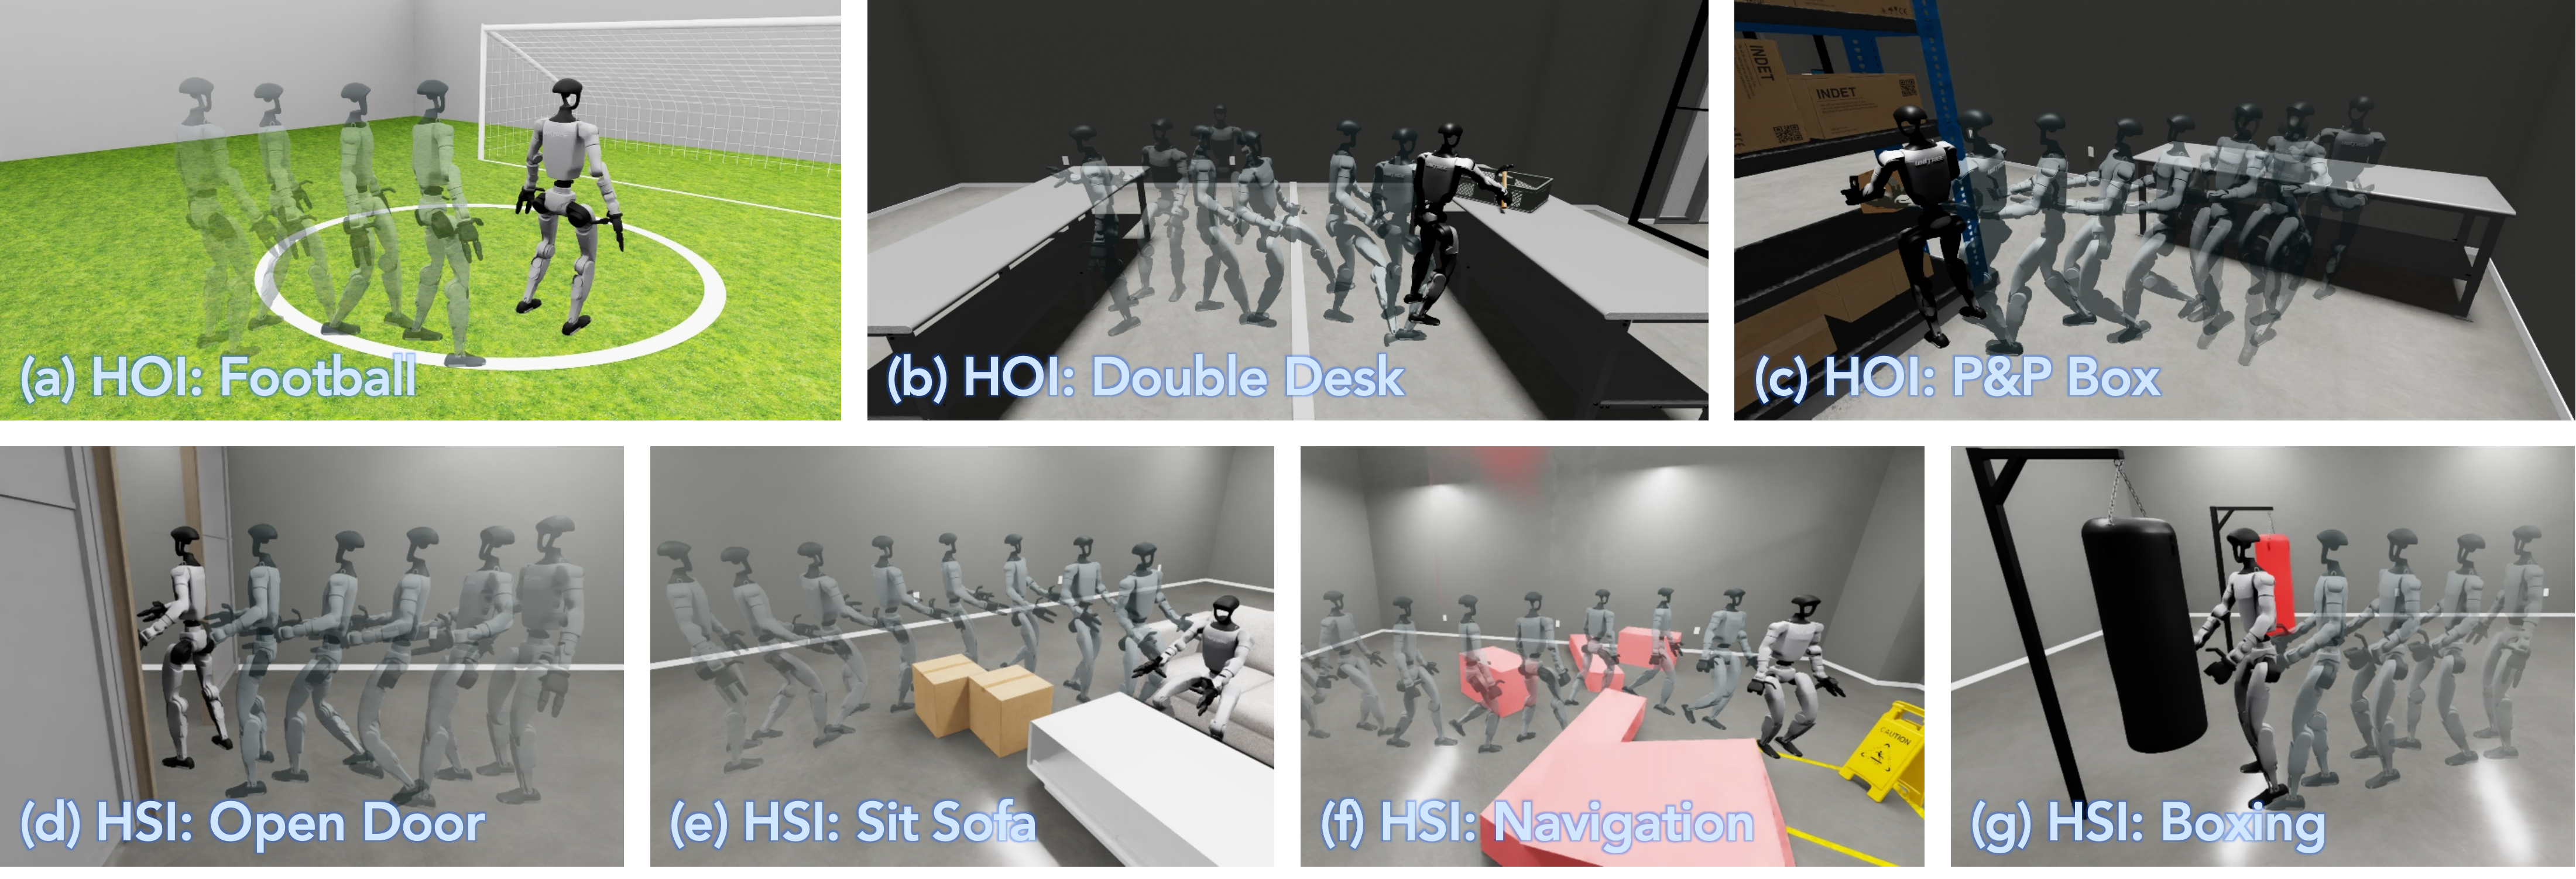
\includegraphics[width=\textwidth]{image/arena.png}
  \caption{\textbf{Visualization of the Seven HumanoidArena Tasks.} The benchmark includes Football, DoubleDesk, P\&Pbox, OpenDoor, SitSofa, Boxing, and VisNavi, covering language-conditioned humanoid behavior across human--object and human--scene interaction with coordinated locomotion, balance, and manipulation.}
  \label{fig:humanoidarena}
\end{figure}

\subsection{SIMPLE Tasks}
\label{sec:vis_simple}

Figure~\ref{fig:simple_tasks} presents the eight evaluated SIMPLE tasks in furnished indoor environments. Handover, Mobile P\&P, and XMoveBendPick combine object handling with positioning relative to the target. CloseDoor, OpenOven, OpenFaucet, and OpenTrashCan involve operating articulated objects, whereas Push Office Chair requires maintaining contact while moving an object through the scene. The panels illustrate variations in target geometry, interaction location, and required body posture. Section~\ref{sec:exp_simple} evaluates these tasks under the L0--L2 protocol to quantify robustness to visual, lighting, and target-pose variation.

\begin{figure}[H]
  \centering
  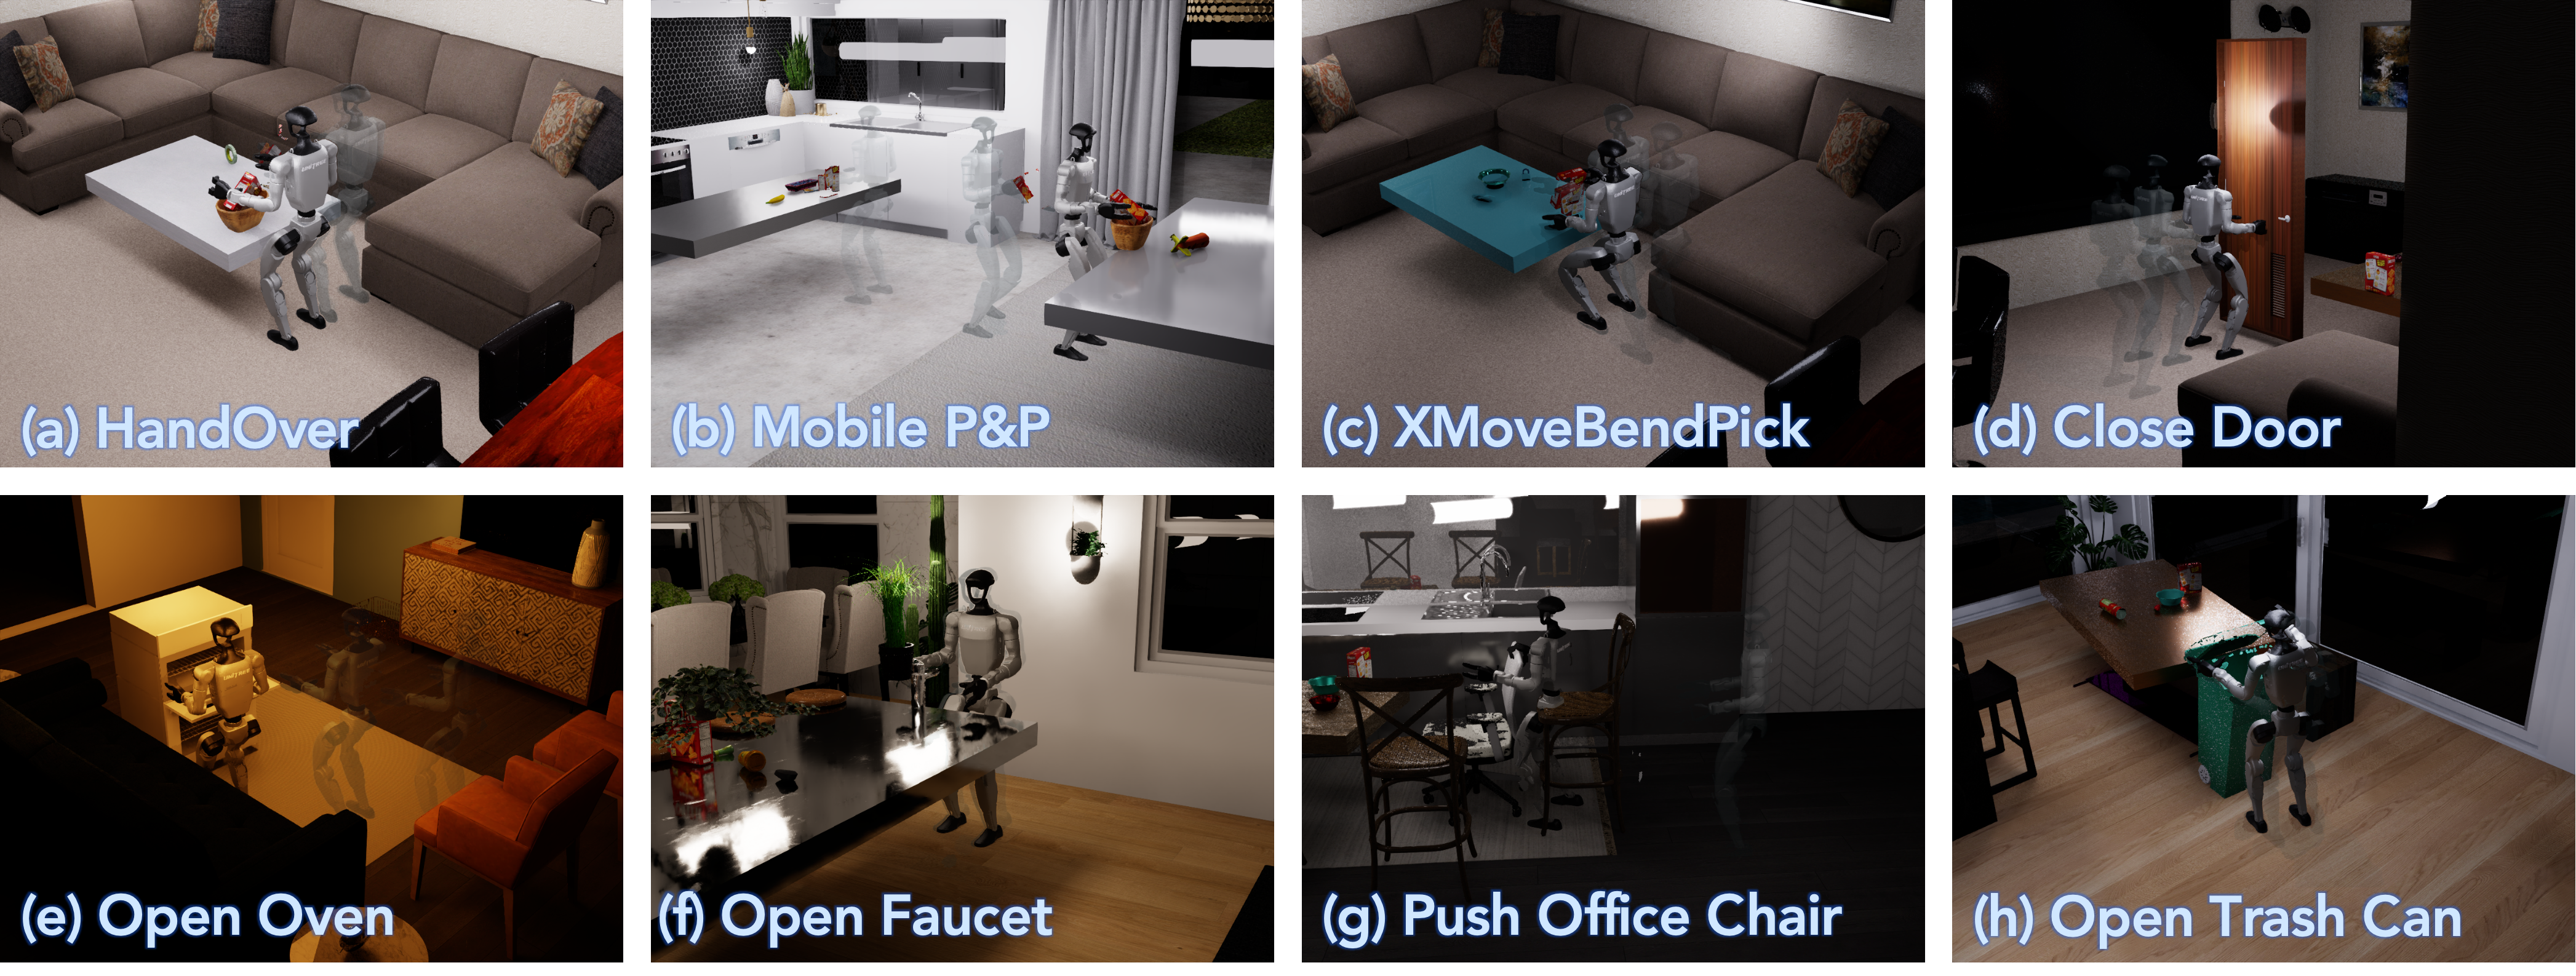
\includegraphics[width=\textwidth]{image/simple.png}
  \caption{\textbf{Evaluated SIMPLE Task Suite.} The selected tasks cover object handover and mobile pick-and-place, locomotion-integrated object pickup, articulated-object interaction, and household-object manipulation. Panels show (a) Handover, (b) Mobile P\&P, (c) XMoveBendPick, (d) CloseDoor, (e) OpenOven, (f) OpenFaucet, (g) Push Office Chair, and (h) OpenTrashCan.}
  \label{fig:simple_tasks}
\end{figure}

\subsection{Real-World Tasks}
\label{sec:vis_real_world}

\begin{figure}[H]
  \centering
  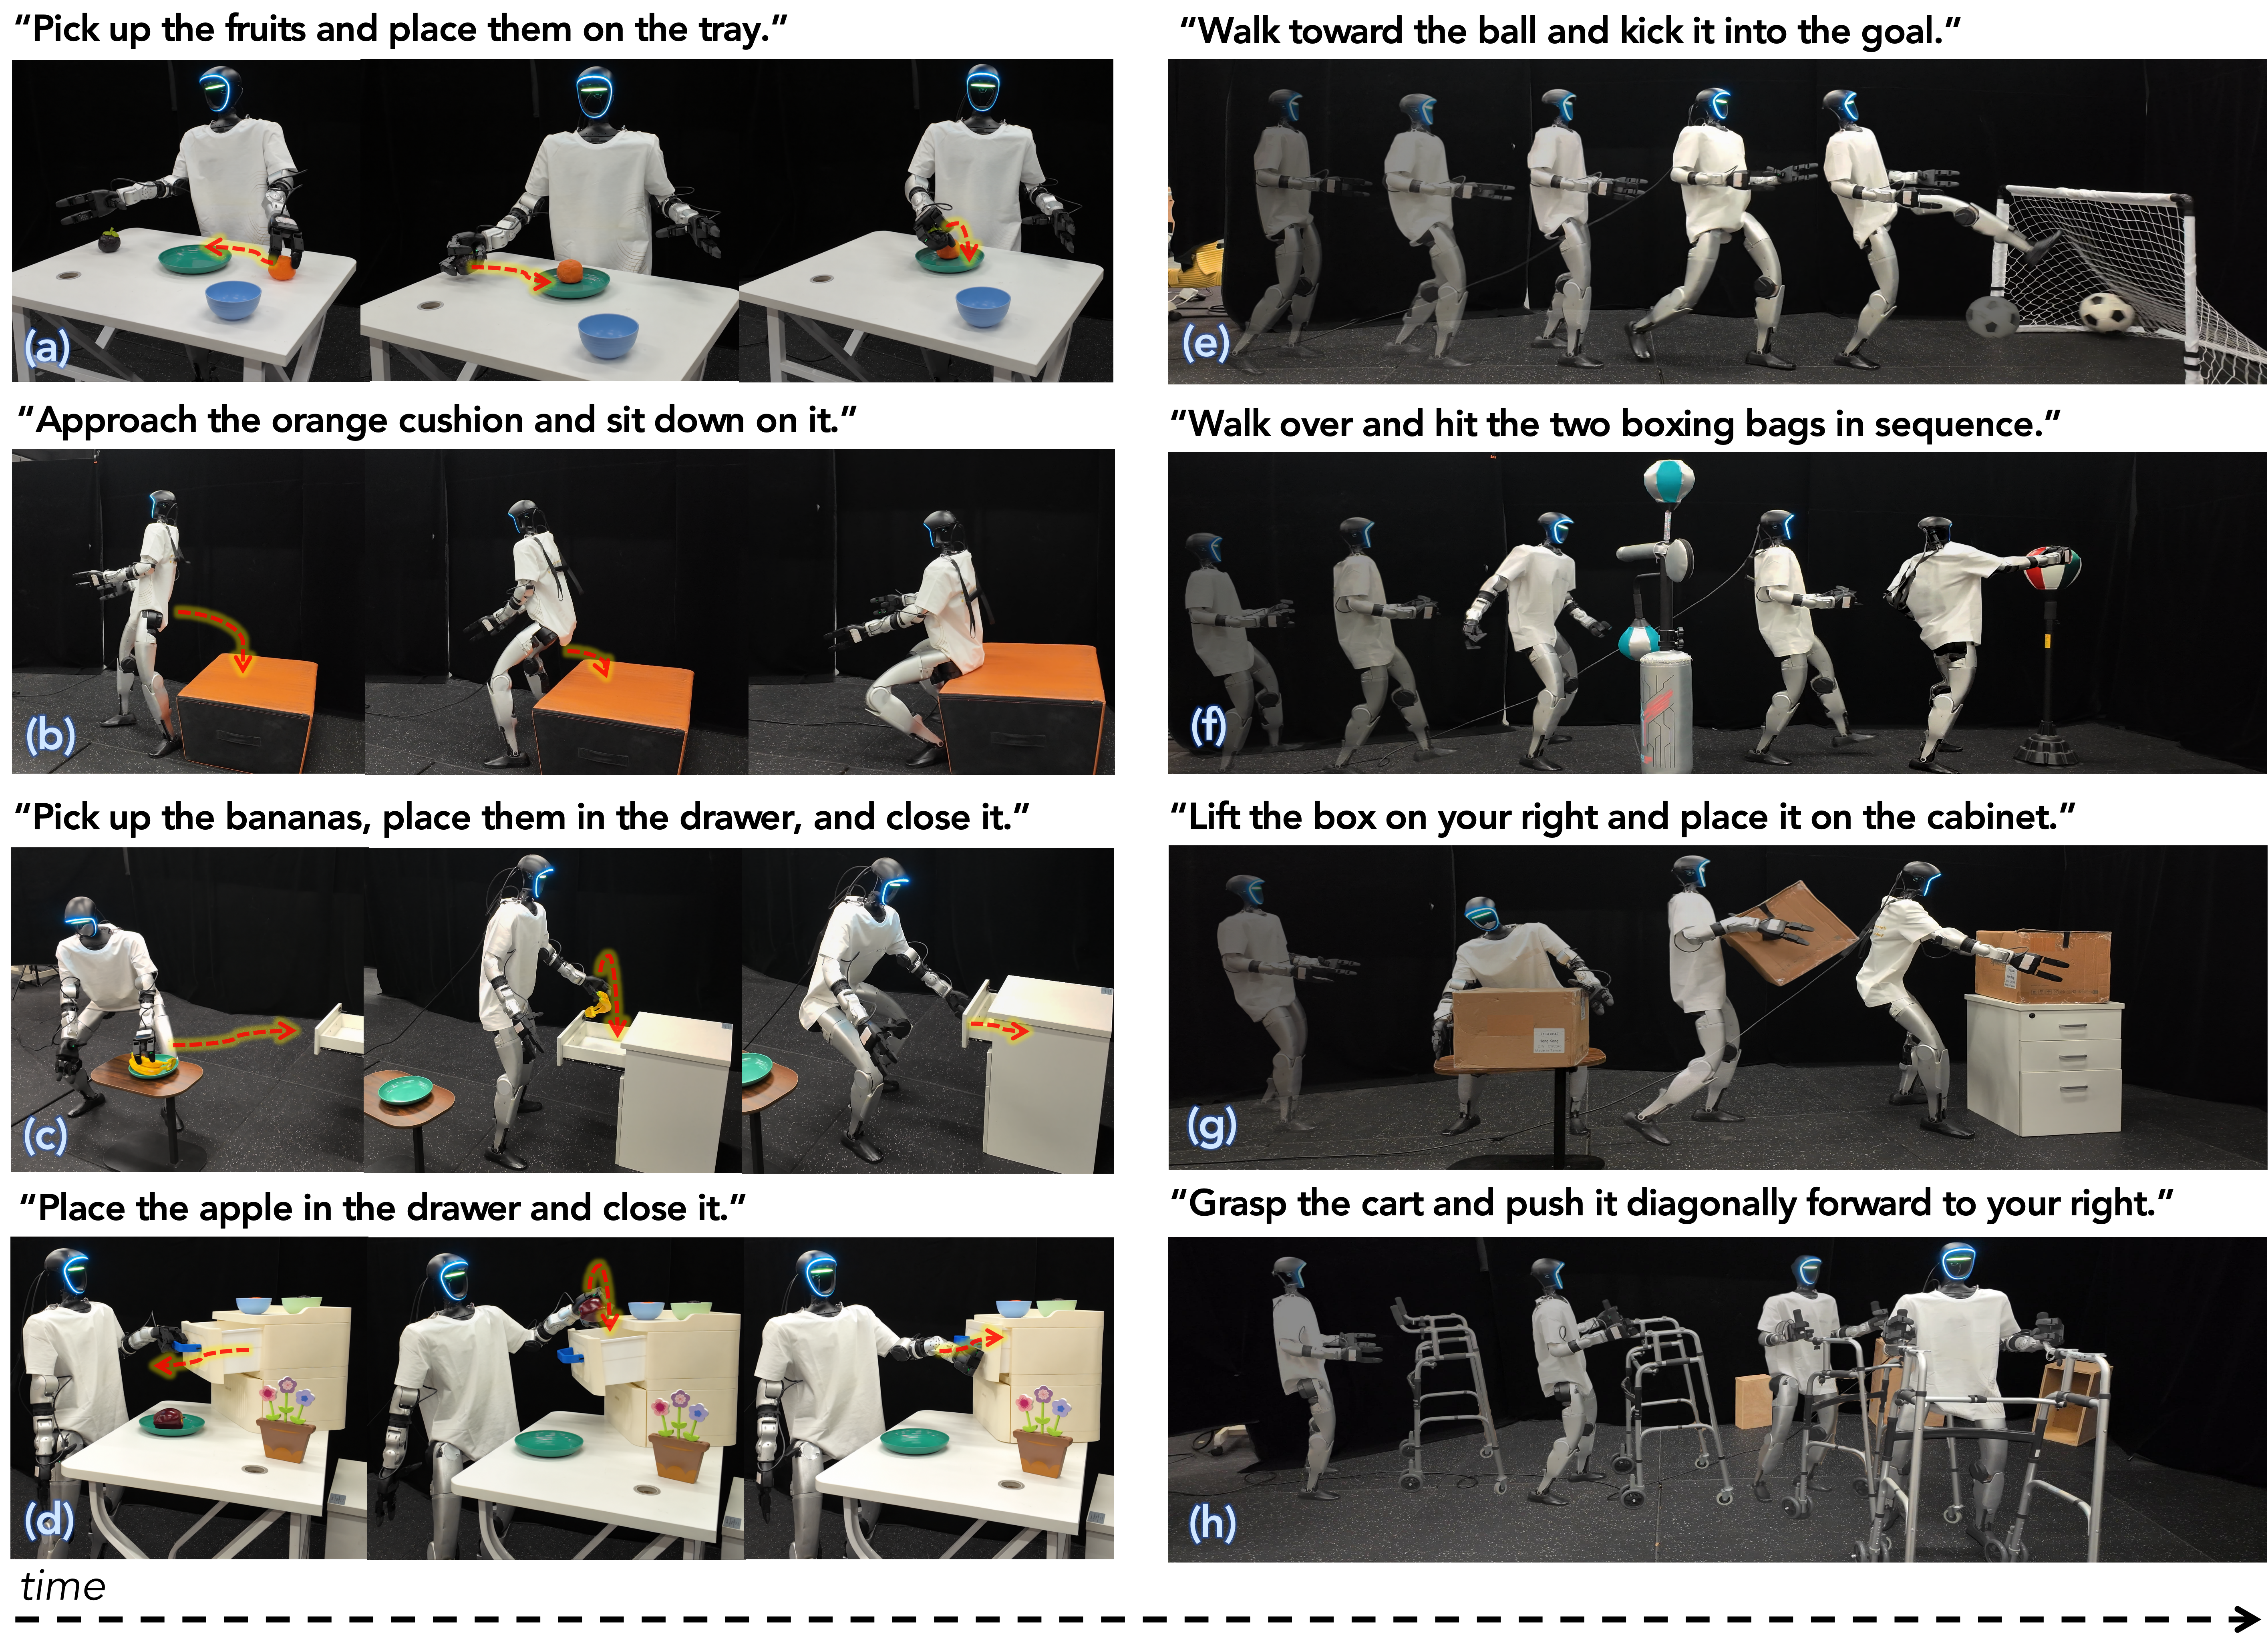
\includegraphics[width=\textwidth]{image/real_world.png}
  \caption{\textbf{Examples of Real-World Humanoid Manipulation.} The image shows representative interaction scenarios involving articulated objects, object transport, and coordinated whole-body motion.}
  \label{fig:real_world}
\end{figure}

Figure~\ref{fig:real_world} presents temporally ordered snapshots of the eight real-world tasks, with language instructions specifying the intended interactions. Panels (a--d) show tabletop pick-and-place, cushion sitting, banana placement followed by drawer closure, and apple placement followed by drawer closure. Panels (e--h) show approaching and kicking a ball, sequential interaction with two punching bags, carrying a box to a cabinet, and pushing a cart. Within each panel, the sequence progresses from preparation or approach to interaction and subsequent motion. The accompanying changes in body posture illustrate the coordination of locomotion, reaching, and sustained contact required by these tasks. Quantitative success rates are reported in Section~\ref{sec:exp_real}.


\section{Extended Motion-Prior Transfer Analysis}
\label{sec:t2m_analysis_appendix}

Table~\ref{tab:t2m_dependency} compares Kimodo-G1-SEED-v1 and RP-v1 under the same policy architecture, adaptation procedure, and HumanoidArena evaluation protocol. Both backbones contain 282M parameters, but use different motion corpora: 288\,h of BONES-SEED and 700\,h of Rigplay, respectively, each with a 90\%/10\% train/test split. Corpus composition and duration therefore change together; this comparison evaluates the choice of pretrained motion prior rather than isolating the effect of data volume.

RP-v1 raises overall success from 64.29\% to 67.63\%, a 3.34-percentage-point gain. Improvements occur on DoubleDesk ($33.33\%\to40.0\%$), P\&Pbox ($75.0\%\to80.0\%$), OpenDoor ($60.0\%\to93.3\%$), and SitSofa ($90.0\%\to96.7\%$). Performance decreases on Football ($50.0\%\to35.0\%$), Boxing ($71.67\%\to66.7\%$), and VisNavi ($70.0\%\to61.7\%$). The largest improvement is on OpenDoor, whereas the remaining changes show that transfer is task-dependent. Thus, a motion prior that improves aggregate performance need not improve every skill.

Table~\ref{tab:t2m_dependency} reports task-level means and standard deviations over three seeds. These descriptive comparisons do not establish statistical significance, particularly for smaller differences relative to the reported variability. The results support the importance of motion-prior selection for downstream control, while leaving the separate contributions of corpus scale, composition, and task coverage unresolved.


\section{Extended Scaling Analysis}
\label{sec:scaling_analysis_appendix}

Figure~\ref{fig:scaling_analysis} examines VLA pretraining data and active policy capacity in separate controlled sweeps. The data sweep holds the architecture, SonicX7 adaptation, and evaluation fixed; the model sweep holds the pretrained T2M backbone, downstream data, optimization, and evaluation fixed. RTC is disabled in both sweeps.

\textbf{Data scaling.} Overall success increases from 68.10\% at 105\,h to 69.05\% at 210\,h and 72.14\% at 419\,h. These approximately twofold increases in data yield successive gains of 0.95 and 3.09 percentage points, totaling 4.04 points. The larger gain in the second interval indicates that additional pretraining data remains beneficial over the tested range. Three operating points, however, do not establish a general scaling law or predict gains beyond 419\,h.

\textbf{Model scaling.} Increasing active policy parameters from 53.6M to 91.7M improves overall success from 61.43\% to 67.63\% (+6.20 points); increasing to 158.9M yields 68.57\% (+0.94 points). The total gain is 7.14 points, with a smaller marginal improvement over the second interval despite a larger parameter increase. This pattern supports increasing policy capacity within the tested range, while suggesting diminishing returns over the sampled sizes. It does not establish a saturation point. Because the two sweeps vary different factors, their gains should be interpreted separately; they do not establish the benefit of jointly scaling data and capacity.


\section{Extended Ablation Analysis}
\label{sec:ablation_analysis_appendix}

All variants train on mixed HumanoidArena tasks in SONIC X7 and evaluate on DoubleDesk, Football, and P\&Pbox. Figure~\ref{fig:training_loss_comparison} reports mean success across these tasks. Each component ablation is compared separately with the 51.67\% baseline without VLA pretraining; the ablations are not cumulative.

\textbf{Motion prior and backbone freezing.}
Removing the pretrained T2M backbone reduces success to 18.33\%, supporting its contribution to whole-body control. Separately, unfreezing the backbone yields 31.67\%, suggesting that preserving pretrained motion representations is beneficial under this adaptation protocol. These comparisons support retaining a frozen motion generator while learning visual and task conditioning through dedicated trainable branches.

\textbf{Prediction objective and gradient decoupling.}
Replacing MSE with Kimodo's original motion objective yields 35.00\% success, compared with 51.67\% for the baseline. This favors direct supervision of policy prediction targets while retaining the pretrained motion prior. Removing root--body gradient detachment instead yields 45.00\%. Detachment preserves root-to-body conditioning but prevents the body loss from updating the root ControlNet, allowing each stage to learn through its own objective while maintaining coordinated generation. The separate comparisons support both the prediction objective and controlled cross-stage gradient flow.

\textbf{VLA pretraining.}
VLA pretraining improves success from 51.67\% to 56.11\%, with generally lower and less variable training loss. Both variants retain the pretrained T2M backbone, so this improvement indicates a complementary benefit from learning visual and task conditioning. Together, the ablations support the evaluated design choices, but do not measure interactions among simultaneous component changes or establish that their individual gains would combine additively.


\section{Limitations and Future Directions}
\label{sec:limitations_future}

\textbf{Limitations.} A principal limitation of the current framework is its dependence on a specific low-level motion tracker. Kimodo-Policy is designed and evaluated with SONIC, and its motion-reference interface and deployment pipeline are tailored to this tracker; other tracking controllers are not currently supported. Consequently, the reported results establish the effectiveness of the policy within the SONIC-based control stack, while transfer across trackers remains unverified. Although separating high-level motion generation from low-level execution provides a modular organization, this separation alone does not ensure compatibility with controllers that differ in reference parameterization, tracking behavior, or executable motion range. Extending the framework would therefore require adapting the policy–tracker interface and validating closed-loop performance under the target controller. Developing a more general interface between pretrained motion generation and low-level whole-body control remains an important direction for broadening its applicability.

\textbf{Future Work.} Looking ahead, Kimodo-Policy can be viewed as a motion-prior-informed action expert within a larger multimodal architecture. Integrating it with vision–language models and video generation models, potentially through MoT-style architectures, could combine semantic understanding and visual dynamics modeling with structured whole-body action generation. A complementary direction is to strengthen the underlying motion prior itself. Text–motion supervision can draw on human motion data retargeted to robot embodiments without requiring every sequence to be collected through robot execution with synchronized visual observations, offering a scalable route to motion pretraining. The gains observed with stronger T2M backbones motivate investigating whether broader motion coverage and more capable generators yield further improvements in downstream control. Beyond training robot-space motion models on retargeted data, a longer-term direction is to transfer pretrained human T2M backbones directly into humanoid VLA policies, drawing on the breadth of human motion resources and advances in human motion generation. Such transfer would require aligning motion representations across embodiments and adapting human kinematic priors to robot-specific actuation, balance, and contact constraints. These directions could expand the framework from a standalone policy into a reusable motion-generation component for more capable humanoid systems.


\clearpage
\bibliographystyle{iclr2027_conference}
\bibliography{ref}
\end{document}
